% ---------------------------------------------------------------------------
\hypertarget{appendix-using-sage}{}
\section{Using Sage with this Script}
\label{s:appendix-using-sage}

This script includes numerous code samples using Sage. Sage is an open
source computer algebra system that supports teaching, study and
research in mathematics.  It combines numerous high-quality open
source packages and provides access to their functionalities via a
common interface, namely, a Python based programming language.  Sage
can be used as a powerful desktop calculator, as a tool to help
undergraduate students study mathematics, or as a programming
environment for prototyping algorithms and research in algorithmic
aspects of mathematics.  With respect to studying cryptography, Sage
modules in the directory  \url{SAGE_ROOT/devel/sage-main/sage/crypto}
can be used to complement a first course in cryptography.  David
Kohel's notes at
\begin{center}
  \url{http://www.sagemath.org/library/crypto.pdf}
\end{center}
can be used to teach such a course that incorporates Sage.


\section*{Sage user interfaces}

Sage is available free of charge and can be downloaded from the
following website:
\begin{center}
  \url{http://www.sagemath.org} \\
\end{center}
The default interface to Sage is command line based, as shown in
Figure~\ref{fig:sage_cmd_interfaces}. However, there is a
graphical user interface to the software as well in the form of the
Sage notebook (see Figure~\ref{fig:sage_gui_interfaces}). We can even
use Sage online at
\begin{center}
\url{http://www.sagenb.org}
\end{center}
without having to install Sage locally. Sage runs under many popular
Linux distributions, Mac OS X, and Windows. For the Windows platform,
a complete distribution of Sage currently only runs as a VMware
image. However, a full native port of Sage to Windows is currently in
progress.

\begin{figure}[!htpb]
\centering
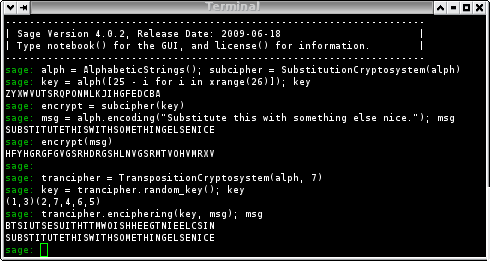
\includegraphics[scale=0.5]{figures/sage-cmd}
\caption{Sage command line interface.}
\label{fig:sage_cmd_interfaces}
\end{figure}

\begin{figure}[!htpb]
\centering
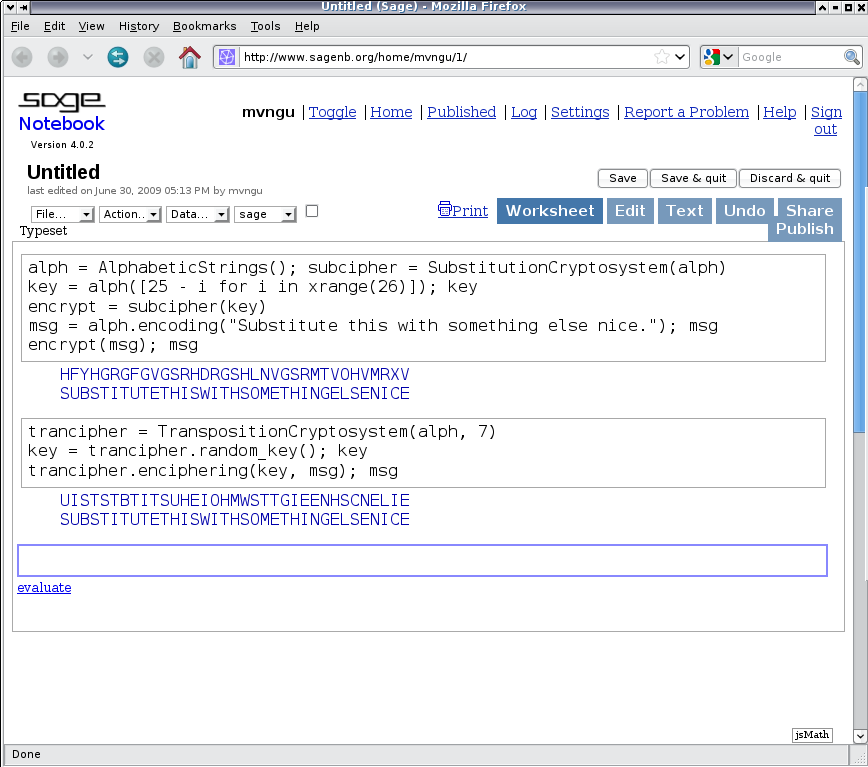
\includegraphics[scale=0.4]{figures/sage-gui}
\caption{Sage notebook interface.}
\label{fig:sage_gui_interfaces}
\end{figure}

\newpage

\section*{Getting help with using Sage}

Upon loading Sage from the command line, we are presented with
something similar to the following:
%
\begin{Verbatim}%
[fontsize=\footnotesize,fontshape=tt]
----------------------------------------------------------------------
| Sage Version 4.0.2, Release Date: 2009-06-18                       |
| Type notebook() for the GUI, and license() for information.        |
----------------------------------------------------------------------
sage:
\end{Verbatim}
%
Plenty of help is provided in the form of the official Sage
documentation that is distributed with every release of Sage~(see
Figure~\ref{fig:sage_standard_doc}).
%
\begin{figure}[!htpb]
\centering
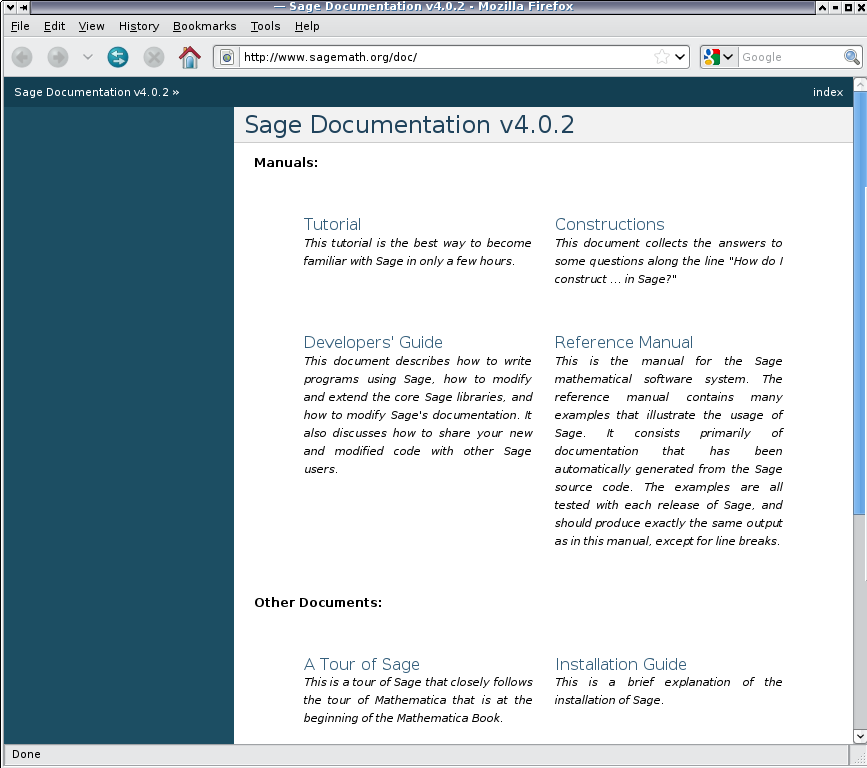
\includegraphics[scale=0.4]{figures/sage-online-doc}
\caption{The Sage standard documentation.}
\label{fig:sage_standard_doc}
\end{figure}
%
The official Sage standard documentation includes the following documents:

\begin{itemize}
\item Tutorial --- This tutorial is designed to help Sage beginners
  become familiar with Sage. It covers many features that beginners
  should be familiar with, and takes one to three hours to go through.

\item Constructions --- This document is in the style of a Sage
  ``cookbook''. It is a collection of answers to questions about
  constructing various objects in Sage.

\item Developers' Guide --- This guide is for developers who want to
  contribute to the development of Sage. Among other issues, it covers
  coding style and conventions, modifying the core Sage libraries,
  modifying the Sage standard documentation, and code review and
  distribution.

\item Reference Manual --- This manual provides complete documentation
  on the major features of Sage. The description of a class is
  accompanied by numerous code samples. All code samples in the
  reference manual are tested before each Sage release.

\item Installation Guide --- This guide explains how to install Sage
  under various platforms.

\item A Tour of Sage --- This is a tour of Sage that showcases various
  features of Sage that are useful for beginners.

\item Numerical Sage --- This document introduces tools available
  under Sage that are useful for numerical computation.

\item Three Lectures about Explicit Methods in Number Theory Using
  Sage --- This document is about using Sage to perform computations
  in advanced number theory.
\end{itemize}

From within a Sage session, we can obtain a list of commands matching
some pattern.  To do so, we type the first few characters and then
press the ``Tab'' key:
%
\begin{Verbatim}%
[fontsize=\footnotesize,fontshape=tt]
sage: Su[TAB]
Subsets                   Subwords                  SuzukiGroup
SubstitutionCryptosystem  SupersingularModule
\end{Verbatim}
%
If we know the exact name of a command, we can use the \texttt{help}
function to obtain further information on that command, or append the
question mark ``?'' to the command name.  For example,
the command \texttt{help(SubstitutionCryptosystem)} provides
documentation on the built-in class
\texttt{SubstitutionCryptosystem}. We can also obtain documentation on
this class as follows:
%
\begin{Verbatim}%
[fontsize=\footnotesize,fontshape=tt]
sage: SubstitutionCryptosystem?
Type:type
Base Class:<type 'type'>
String Form:<class 'sage.crypto.classical.SubstitutionCryptosystem'>
Namespace:Interactive
File:/home/mvngu/usr/bin/sage-3.4.1/local/lib/python2.5/site-packages/sage/crypto/classical.py
Docstring:

        Create a substitution cryptosystem.

        INPUT:

        - ``S`` - a string monoid over some alphabet

        OUTPUT:

        - A substitution cryptosystem over the alphabet ``S``.

        EXAMPLES::

            sage: M = AlphabeticStrings()
            sage: E = SubstitutionCryptosystem(M)
            sage: E
            Substitution cryptosystem on Free alphabetic string monoid
            on A-Z
            sage: K = M([ 25-i for i in range(26) ])
            sage: K
            ZYXWVUTSRQPONMLKJIHGFEDCBA
            sage: e = E(K)
            sage: m = M(``THECATINTHEHAT'')
            sage: e(m)
            GSVXZGRMGSVSZG

        TESTS::

            sage: M = AlphabeticStrings()
            sage: E = SubstitutionCryptosystem(M)
            sage: E == loads(dumps(E))
            True
\end{Verbatim}
%
For further assistance on specific problems, we can also
search the archive of the \texttt{sage-support} mailing list at
%
\begin{center}
  \url{http://groups.google.com/group/sage-support}
\end{center}
